\section*{Sposoby ewaluacji}

\section*{Porównanie z Stockfish}
Najbardziej obiektywnym sposobem oceny działania algorytmu szachowego jest porównanie go z innym, popularnym silnikiem szachowym. Do porównania został wybrany Stockfish, ze względu na jego pupularność oraz wsparcie biblioteki chess do jego integracji. 

Porównanie polega na rozegraniu podanej liczby partii pomiędzy dwoma silnikami. Białe figury są reprezentowane przez Stockfish, a czarne przez opisywany model. Główną miarą oceny jest przeżywalność, czyli liczba ruchów w danej partii. Dodatkowo w celu uzyskania bardziej szczegółowych danych, stockfish w każdej rundzie podaje ocenę pozycji dla czarnych figur. Mieści się ona w przedziale od -1000 do 1000, gdzie skrajne wartości oznaczają mat.
Użytkownik poza wybraniem liczby partii, może również ustawić w pliku konfiguracyjnym ilość najlepszych generowanych ruchów, z których jest losowany ostateczny ruch czarnych. Taki mechanizm został zastosowany w celu obniżenia poziomu trudności oraz zwiększenia losowości rozgrywki. Takie podejście pozwala uwypuklić różnice pomiędzy dwoma silnikami. Aby uzyskać bardziej powtarzalne wyniki podczas porównywania sieci neuronowych, w pliku konfiguracyjnym można również ustawić ziarno generatora liczb pseudolosowych.

Na wykresie przedstawiającego dane, jest również zaznaczony wynik losowego gracza, który w każdej turze wykonuje losowy prawidłowy ruch. Pozwala to na ocenę, czy dany model w ogóle działa.

\begin{figure}[h]
\centering
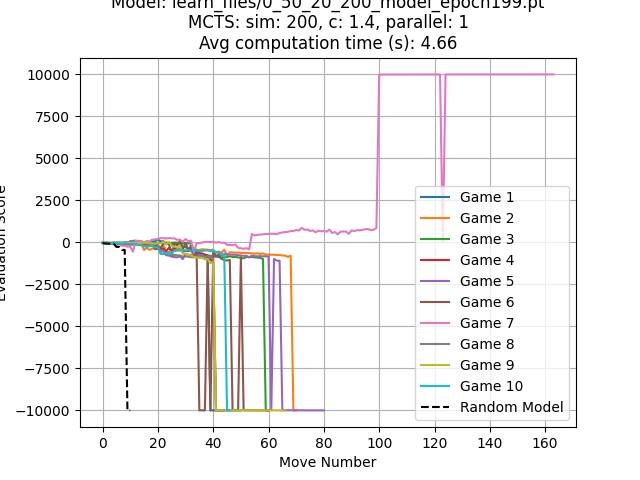
\includegraphics[width=0.6\textwidth]{images/eval_stock_example.png}
\caption{Przykładowy wykres porównania z Stockfish}
\end{figure}

\section*{Macierz omyłek}
Macierz omyłek jest podstawowym narzędziem do analizy modelu. Została ona zastosowana tylko dla value network, gdyż (todo: dopisać/przetestować). Jest ona obliczana na podstawie danych testowych. Obliczane są również miary takie jak precyzja, czułość oraz F1.


\section*{Wykres Loss}
Wykres loss przedstawia różnicę pomiędzy przewidywaniami modelu, a rzeczywistymi wartościami dla każdej epoki. W celu przyśpieszenia obliczeń, wraz z modelem jest zapisywana również wartość loss dla danych treningowych. Podczas tworzenia wykresu są obliczane wartości tylko dla danych testowych. Wraz ze wzrostem liczby epok oraz wielkości zbioru testowego, czas tworzenia wykresu rośnie. Z tego powodu została wprowadzona zmienna \textit{skip factor}, która określa co ile epok jest obliczana wartość loss. Pozwala to na ustawienie dokładności wykresu, a co za tym idzie skrócenie czasu jego tworzenia.